\documentclass[dvipsnames, svgnames, x11names, handout]{beamer}
\usepackage[T1]{fontenc}
\usepackage{bold-extra}
\usepackage{amsfonts, amsthm, amsmath, amssymb}
\usepackage{mathtools}
\usepackage{ulem}
\usepackage{bm}
\usepackage{minted}
\usemintedstyle{vs}
\usetheme{Madrid}
\usecolortheme{default}
\usepackage{multirow, multicol}
\usepackage{tikz, pgfplots}
\usetikzlibrary{arrows.meta, math, calc, quotes, intersections, angles, trees, shapes.geometric}
\pgfplotsset{compat=1.18}
\tikzstyle{block} = [rectangle, minimum width=4cm, minimum height=2cm, text centered, draw = black]
\tikzmath{\x1 = 2.5; \y1 = 3;}

\graphicspath{{../images}}

\title[HKUST Future-Ready Scholars]{HKUST Future-Ready Scholars}
\subtitle{Introduction to Game Programming using Python}
\author[Game Programming using Python]{Part 1: Number Guessing Game}
\date[April 2024]{20 April 2024}
\titlegraphic{
\includegraphics[height=1cm]{ust.png}}

\begin{document}

\frame{\titlepage}

\begin{frame}[fragile]{Google Colab}
    \begin{center}
        We will use Google Colab for the workshops.

        \href{https://colab.research.google.com/}{https://colab.research.google.com/}

        You must have a Gmail account for it, create one if you do not.
    \end{center}
\end{frame}

\begin{frame}[fragile]{Files}
    \begin{center}
        All materials today are at:

        \href{https://bit.ly/ustidpo}{https://bit.ly/ustidpo}

        \

        \frame{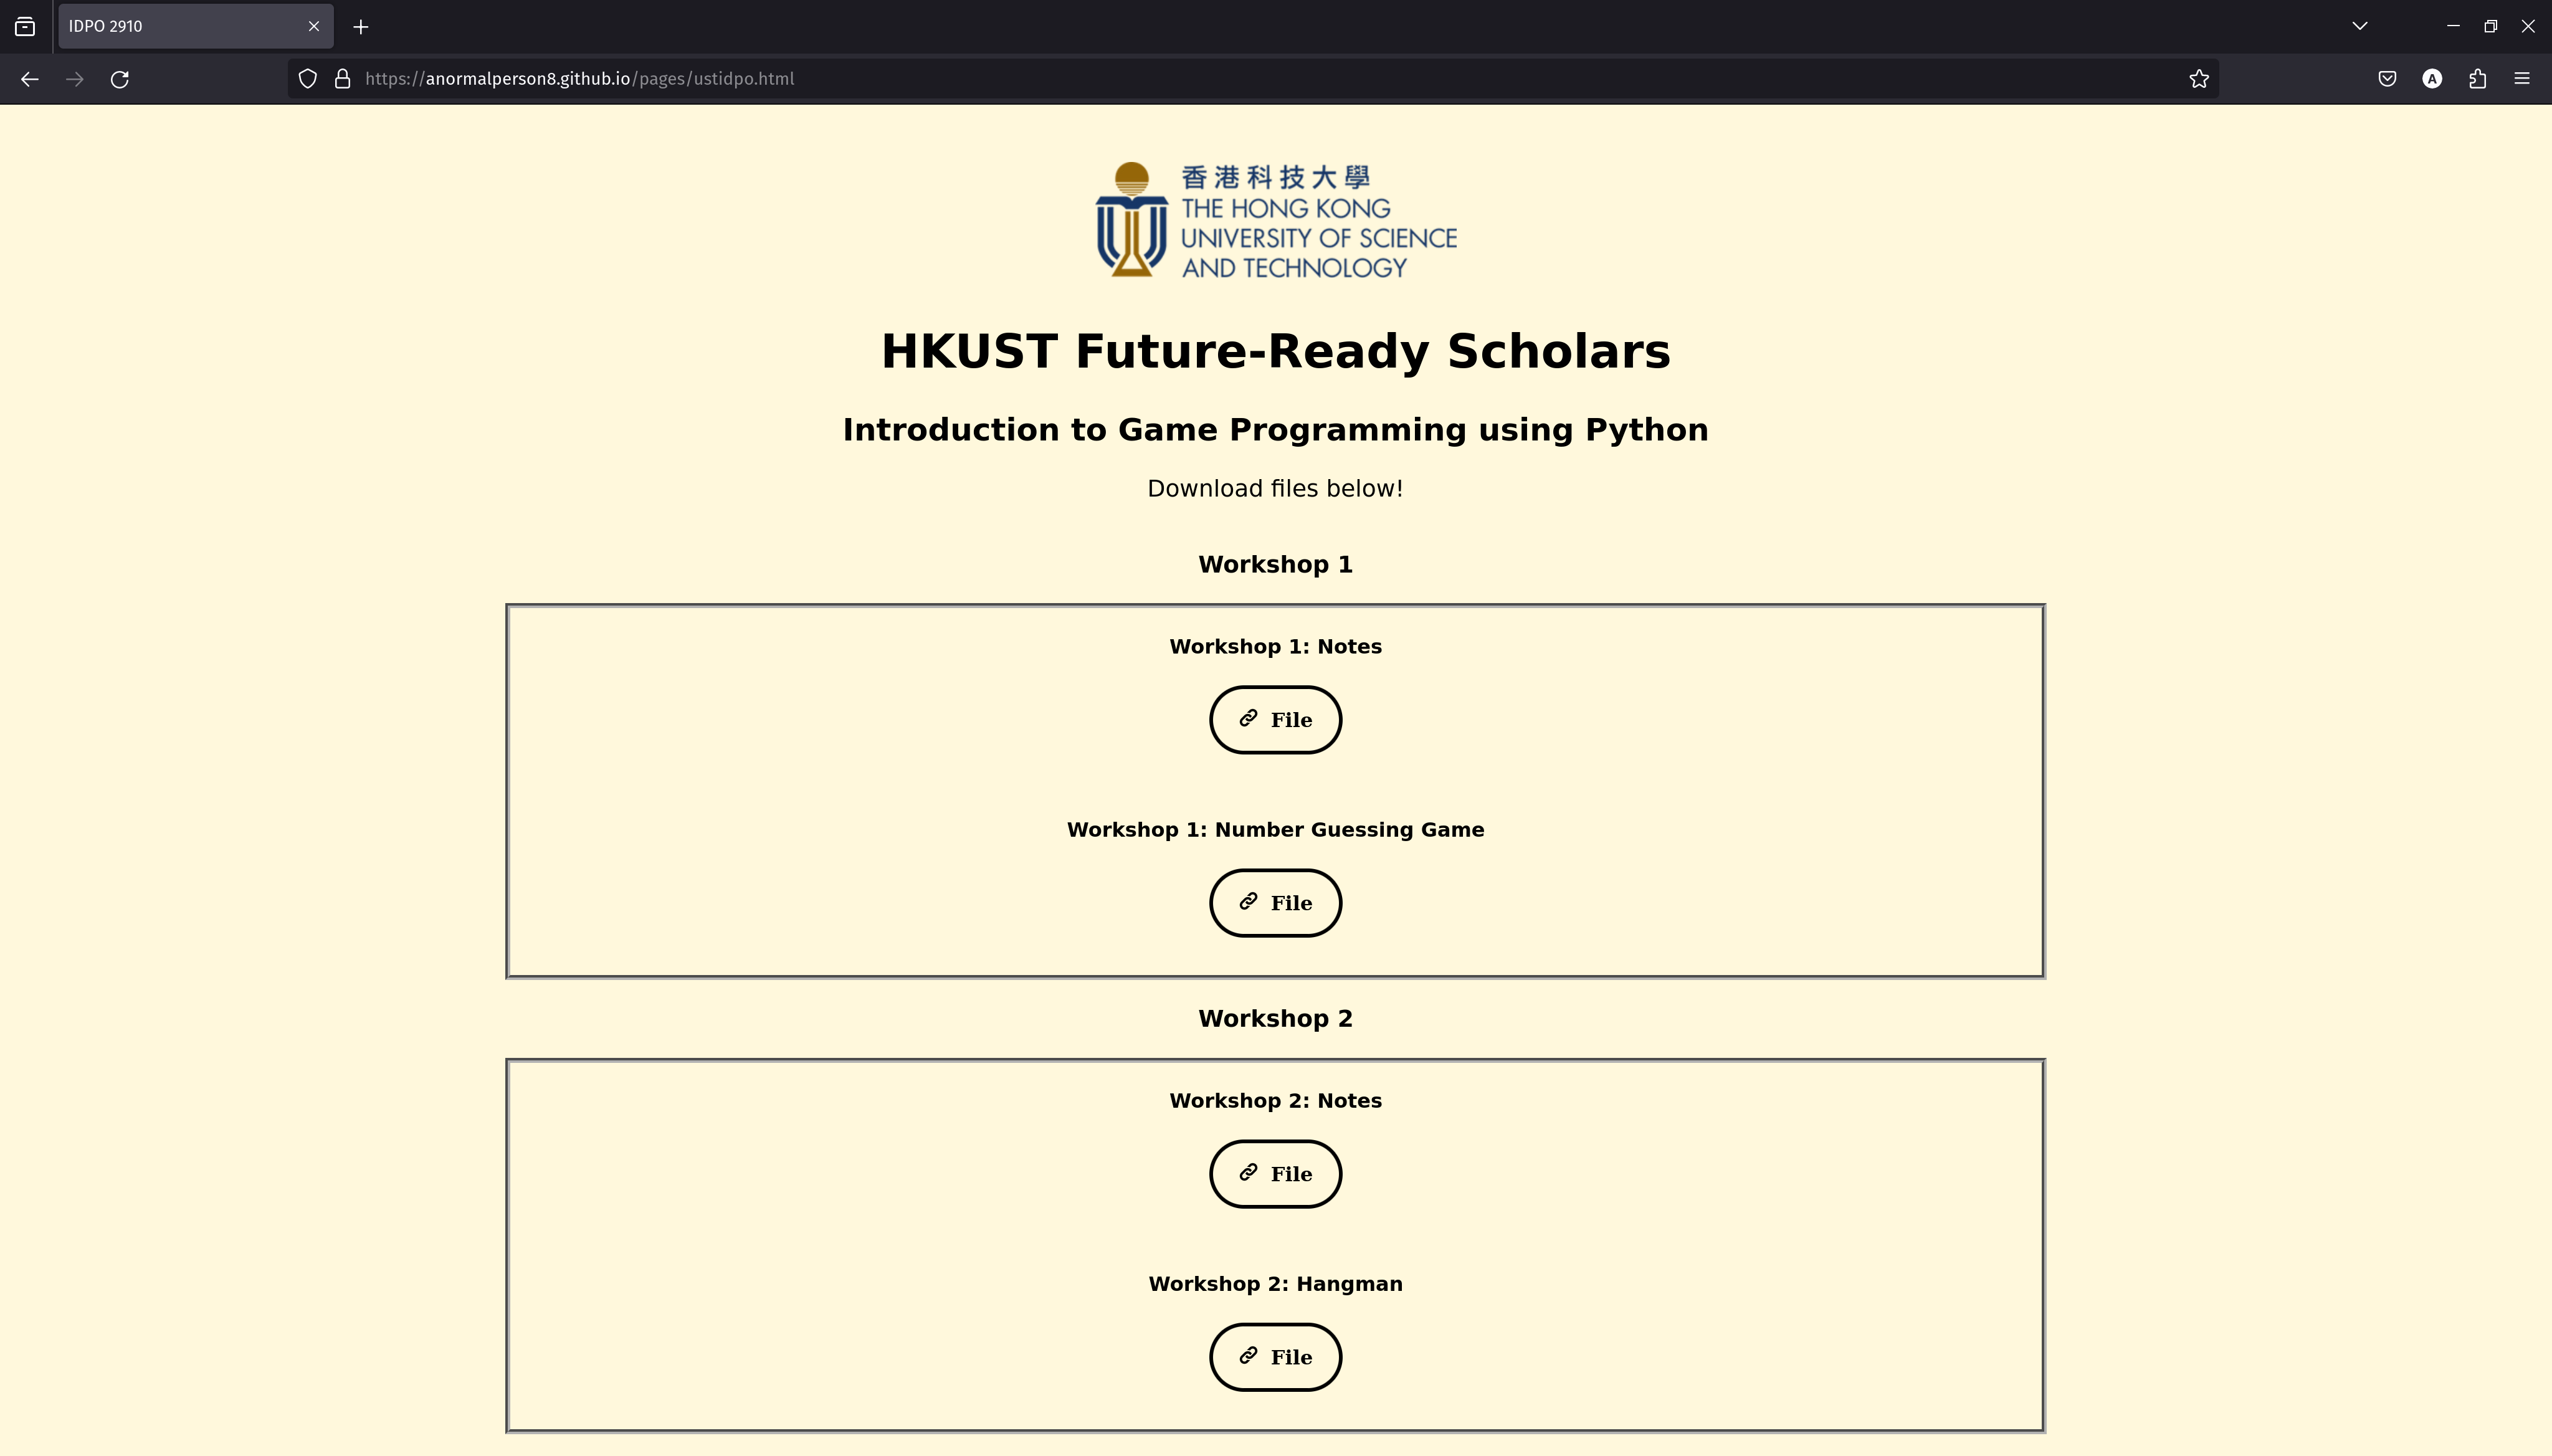
\includegraphics[width=0.75\textwidth]{Download.png}}

        Download all files that belong to \textbf{Workshop 1} today.
    \end{center}
\end{frame}

\begin{frame}[fragile]{Jupyter Notebook}
    \begin{center}
        Now upload your Jupyter Notebook file with \textbf{Files $\rightarrow$ Open Notebook}.
    
        \

        \frame{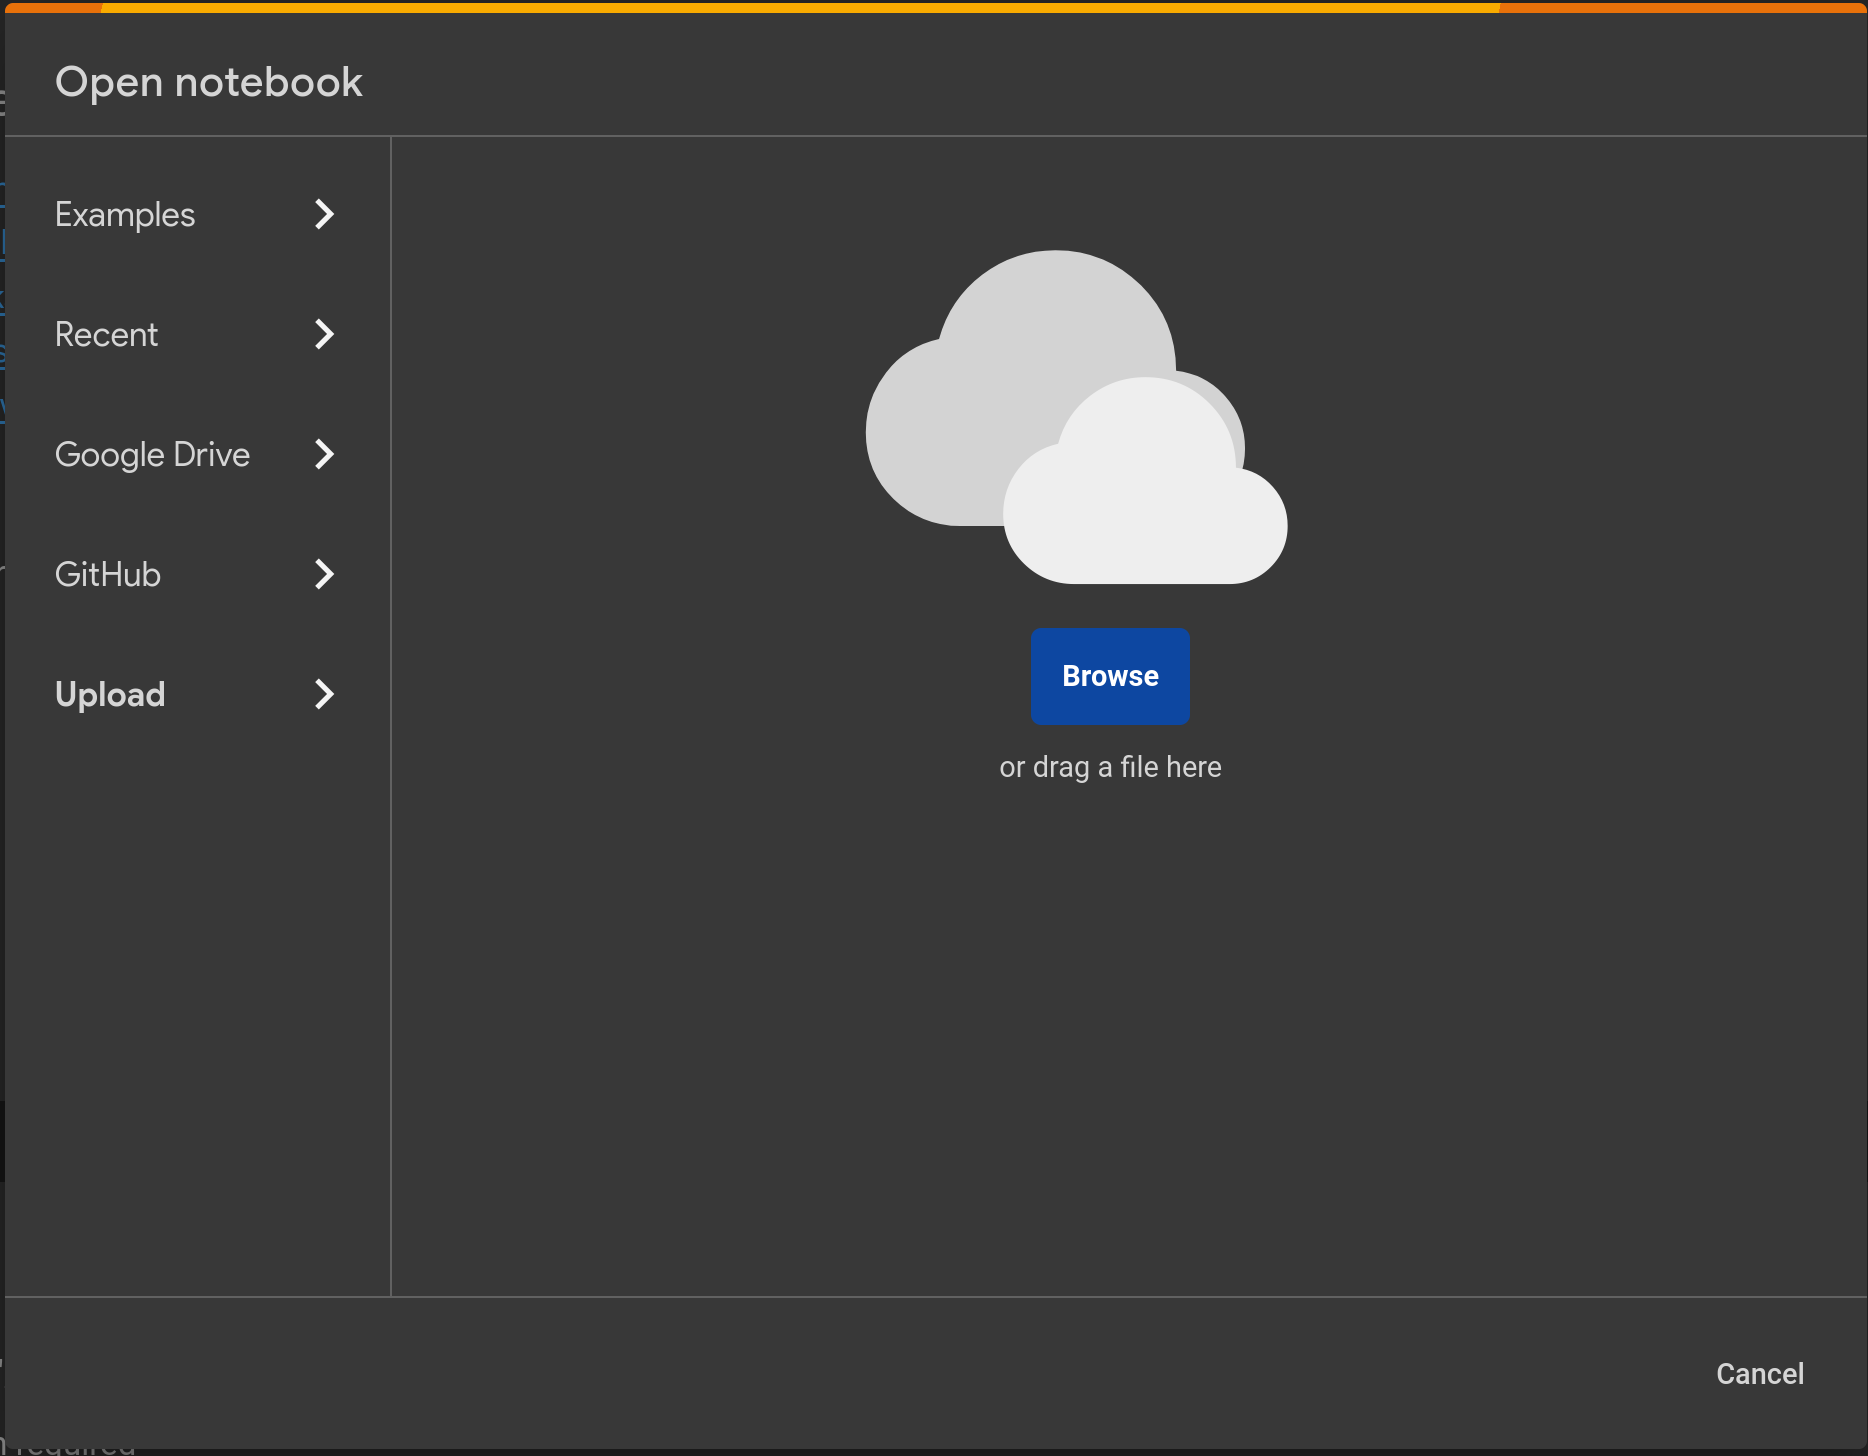
\includegraphics[width=0.5\textwidth]{Upload.png}}

        Upload the file \textbf{Number-Guessing.ipynb}.
    
    \end{center}
\end{frame}

\begin{frame}[fragile]{Using Jupyter Notebook}
    You can type your code in these blocks. We call these blocks code cells.

    \begin{center}
        \frame{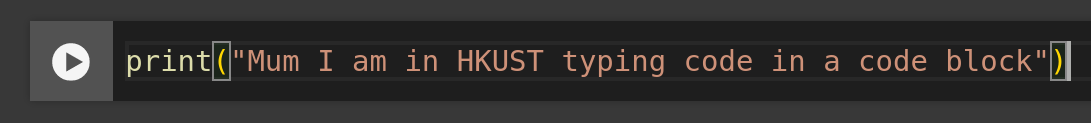
\includegraphics[width=0.5\textwidth]{Use1.png}}
    \end{center}

    \

    You can run a code cell with the button on the left.

    \begin{center}
        \frame{
\includegraphics[width=0.5\textwidth]{Use2.png}}
    \end{center}
\end{frame}

\begin{frame}{World of Game Coding}
    \tikzstyle{block} = [rectangle, minimum width=4cm, minimum height=2cm, text centered, draw = black]
    \tikzmath{\x1 = 2.5; \y1 = 3;}
    
    \hspace{0.2\textwidth}\scalebox{0.5}{\begin{tikzpicture}
    \node (root) [block, fill = Cornsilk2] {Game (Software)};
    \node (program) [block, fill = LightSteelBlue] at ($(root) + (-\x1, -\y1)$) {Program (Codes)};
    \node (mm) [block, fill = Cornsilk2] at ($(root) + (\x1, -\y1)$) {Multimedia};
    
    \node (func) [block, fill = LightSteelBlue] at ($(program) + (0, -\y1)$) {Functions};
    
    \node (if) [block, fill = LightSteelBlue] at ($(func) + (-\x1, -\y1)$) {Decision Making};
    \node (loop) [block, fill = LightSteelBlue] at ($(func) + (\x1, -\y1)$) {Loops};
    
    \node (io) [block, fill = LightSteelBlue] at ($(if) + (0, -\y1)$) {Input/Output};
    \node (var) [block, fill = LightSteelBlue] at ($(loop) + (0, -\y1)$) {Variables};
    
    \draw [->] (root.south) -- ++(0, -0.5) -- ++(-\x1, 0) -- (program.north);
    \draw [->] (root.south) -- ++(0, -0.5) -- ++(\x1, 0) -- (mm.north);
    
    \draw [->] (program.south) -- (func.north);
    
    \draw [->] (func.south) -- ++(0, -0.5) -- ++(-\x1, 0) -- (if.north);
    \draw [->] (func.south) -- ++(0, -0.5) -- ++(\x1, 0) -- (loop.north);
    
    \draw [->] (loop.south) -- ++(0, -0.5) -- ++(-2*\x1, 0) -- (io.north);
    \draw [->] (if.south) -- ++(0, -0.5) -- ++(2*\x1, 0) -- (var.north);
    \end{tikzpicture}}
    
\end{frame}

\begin{frame}{What is Python?}
    Did you know? Python was made by someone who was bored.
    
    It's a language designed to be almost as understandable as English.
    
    You will be using Python 3. Why? Because Python 1 are 2 are too old.
    \begin{center}
    \includegraphics[height=1.5cm]{python-logo.png}\\
    This is the logo of Python.
    \end{center}
\end{frame}
    
\begin{frame}{Contents} 
\begin{center}
    \scalebox{0.5}{\begin{tikzpicture}
    \node (program) [block, fill = LightSteelBlue] {Program (Codes)};
    
    \node (func) [block, fill = LightSteelBlue] at ($(program) + (0, -\y1)$) {Functions};
    
    \node (if) [block, fill = LightSteelBlue] at ($(func) + (-\x1, -\y1)$) {Decision Making};
    \node (loop) [block, fill = LightSteelBlue] at ($(func) + (\x1, -\y1)$) {Loops};
    
    \node (io) [block, fill = DarkSeaGreen2] at ($(if) + (0, -\y1)$) {Input/Output};
    \node (var) [block, fill = LightSteelBlue] at ($(loop) + (0, -\y1)$) {Variables};
    
    \draw [->] (program.south) -- (func.north);
    
    \draw [->] (func.south) -- ++(0, -0.5) -- ++(-\x1, 0) -- (if.north);
    \draw [->] (func.south) -- ++(0, -0.5) -- ++(\x1, 0) -- (loop.north);
    
    \draw [->] (loop.south) -- ++(0, -0.5) -- ++(-2*\x1, 0) -- (io.north);
    \draw [->] (if.south) -- ++(0, -0.5) -- ++(2*\x1, 0) -- (var.north);
    \end{tikzpicture}}
\end{center}
\end{frame}

\begin{frame}[fragile]{The first thing in Python - \texttt{print()} function}

\begin{minted}[tabsize=4]{python} 
print("This is the print function.")
\end{minted}
\end{frame}
    
\begin{frame}[fragile]{The first thing in Python - \texttt{print()} function}
\texttt{print()} is a function that lets you print something,\\
also known as text output.
\begin{minted}[tabsize=4]{python}
print("Word") # This prints the word "Word".
\end{minted}
\vspace{1em}
Examples:
\begin{minted}[tabsize=4]{python} 
>>> print("Hello World")
Hello World
>>> print("Haha hehe")
Haha hehe
\end{minted}
\end{frame}

\begin{frame}[fragile]{Printing multiple things}
You can use a comma (\texttt{,}) to separate different things with a space.
\begin{minted}[tabsize=4]{python} 
>>> print("Alpha", "Beta", "Gamma")
Alpha Beta Gamma
>>> print("Haha", "hehe")
Haha hehe
\end{minted}
\end{frame}

\begin{frame}{Contents}

\begin{center}\scalebox{0.5}{
\begin{tikzpicture}
\node (program) [block, fill = LightSteelBlue] {Program (Codes)};

\node (func) [block, fill = LightSteelBlue] at ($(program) + (0, -\y1)$) {Functions};

\node (if) [block, fill = LightSteelBlue] at ($(func) + (-\x1, -\y1)$) {Decision Making};
\node (loop) [block, fill = LightSteelBlue] at ($(func) + (\x1, -\y1)$) {Loops};

\node (io) [block, fill = LightSteelBlue] at ($(if) + (0, -\y1)$) {Input/Output};
\node (var) [block, fill = DarkSeaGreen2] at ($(loop) + (0, -\y1)$) {Variables};

\draw [->] (program.south) -- (func.north);

\draw [->] (func.south) -- ++(0, -0.5) -- ++(-\x1, 0) -- (if.north);
\draw [->] (func.south) -- ++(0, -0.5) -- ++(\x1, 0) -- (loop.north);

\draw [->] (loop.south) -- ++(0, -0.5) -- ++(-2*\x1, 0) -- (io.north);
\draw [->] (if.south) -- ++(0, -0.5) -- ++(2*\x1, 0) -- (var.north);
\end{tikzpicture}}
\end{center}

\end{frame}

\begin{frame}[fragile]{Variables}
\begin{center}
Imagine you borrow a box from the computer.

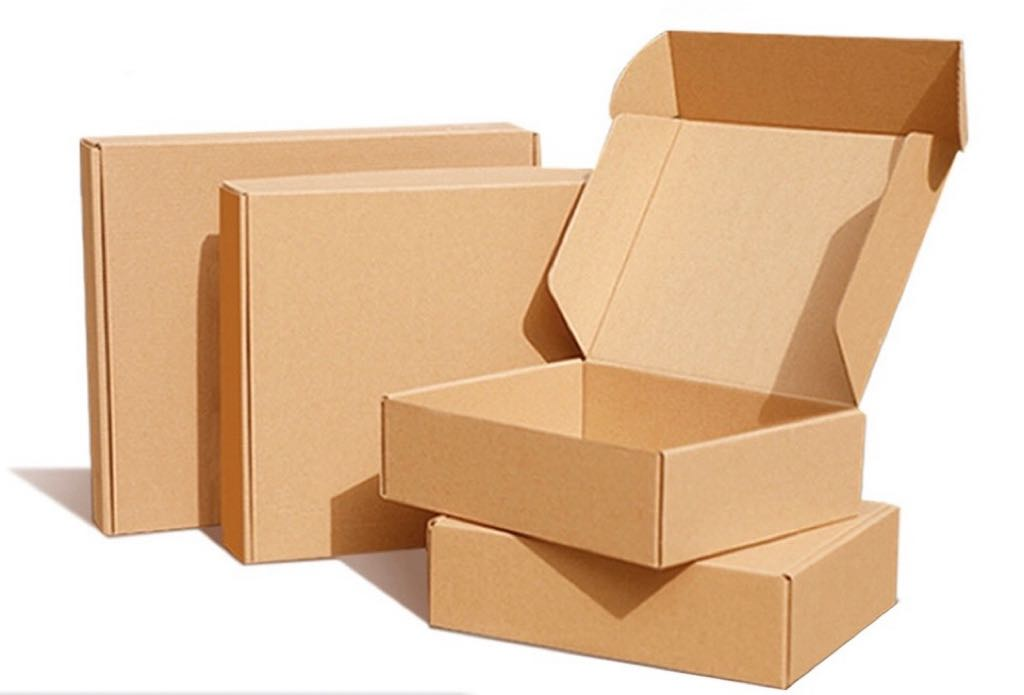
\includegraphics[height=3cm]{box}

\pause
Give it a name and a value, you can now recall this value with the name!
\end{center}
\end{frame}

\begin{frame}[fragile]{Variables}
The code usually goes:\\
\texttt{variable\char`\_name = data}\\
This means whatever \texttt{data} is, it is now stored in a variable with name \texttt{variable\char`\_name}.
\vspace{1em}\\
Some basic variable types:
\begin{minted}[tabsize=4, escapeinside=||]{python}
a = 5       |\pause|# This is an integer (int) stored in a |\pause|
b = True    |\pause|# This is a boolean (bool) stored in b |\pause|
c = 3.2     |\pause|# This is a float (float)  stored in c |\pause|
d = "abc"   |\pause|# This is a string (str)   stored in d |\pause|
e = 'abc'   |\pause|# This is also a string    stored in e
\end{minted}
\end{frame}

\begin{frame}[fragile]{Variables - Integers}
What are integers?\pause\\
Integers are just like what you've learnt in Maths, numbers without decimal points. Are the following valid?\pause
\begin{minted}[tabsize=4, escapeinside=||]{python}
a = 5       |\pause|# Valid|\pause|
b = 12      |\pause|# Valid|\pause|
c = 69420   |\pause|# Valid|\pause|
d = -1984   |\pause|# Valid|\pause|
e = 32.5    |\pause|# This would become a float instead|\pause|
f = '5'     |\pause|# This would become a string instead
\end{minted}
\end{frame}

\begin{frame}[fragile]{Variables - Integer Arithmetic Operations}
You can do normal operations on integers:
\begin{minted}[tabsize=4, escapeinside=||]{python}
a = 1 + 2   |\pause|# a stores the integer 3|\pause|
b = 80 - 52 |\pause|# b stores the integer 28|\pause|
c = 69 * -2 |\pause|# c stores the integer -138|\pause|
d = 6 / 4   |\pause|# d stores the float 1.5|\pause|
e = 18 / 2  |\pause|# e stores the float 9.0|\pause|
\end{minted}
\begin{alertblock}{Division in Python}
Whether a number can be precisely divided or not, division returns a \texttt{float}.
\end{alertblock}
\end{frame}

\begin{frame}[fragile]{Variables - Integer Arithmetic Operations}
Operations with variables:
\begin{minted}[tabsize=4, escapeinside=||]{python}
a = 100
b = 12 |\pause|
c = a + b   |\pause|# c stores the integer 112|\pause|
d = b - a   |\pause|# d stores the integer -88|\pause|
e = a * -b  |\pause|# e stores the integer -1200|\pause|
f = a / b   |\pause|# f stores the float 8.333333333333334
\end{minted}
\end{frame}

\begin{frame}[fragile]{Variables - Integer Arithmetic Operations}
Then how do we get an integer output?\pause
\begin{minted}[tabsize=4, escapeinside=||]{python}
a = 100
b = 12 |\pause|
c = a // b  |\pause|# c stores the integer 8|\pause|
            # // operator takes the closest and smaller 
            # integer from the division operation|\pause|
d = a % b   |\pause|# d stores the integer 4|\pause|
            # % operator takes the remainder of a 
            # division operation
\end{minted}
\end{frame}

\begin{frame}[fragile]{Variables - Integer Arithmetic Operations}
Also, the power (exponent) operation:
\begin{minted}[tabsize=4, escapeinside=||]{python}
a = 2
b = 5       |\pause|
c = a ** b  |\pause|# c stores the integer 32
            # ** operator means power
\end{minted}
\end{frame}
    
\begin{frame}[fragile]{Variables - Floats}
What are floats?\pause\\
Floats are numbers with decimal points.\pause\\
Arithmetic operators we learnt can be applied as well.
\begin{minted}[tabsize=4, escapeinside=||]{python}
a = 0.2     # a stores the float 0.2
b = 3.0     # b stores the float 3.0|\pause|
c = a + b   |\pause|# c stores the float 3.2|\pause|
d = b / a   |\pause|# d stores the float 15.0|\pause|
e = a ** b  |\pause|# e stores the float 0.008000000000000002|\pause|
\end{minted}
\begin{alertblock}{Inaccuracies}
Inaccuracies happen with decimals in Python. Be careful when dealing with floats.
\end{alertblock}
\end{frame}

\begin{frame}[fragile]{Variables - Floats}
What happens when you combine floats and integers? \pause
\begin{minted}[tabsize=4, escapeinside=||]{python}
a = 0.2     # a stores the float 0.2
b = 3       # b stores the integer 3|\pause|
c = a + b   # c stores the float 3.2
d = b / a   # d stores the float 15.0
e = a ** b  # e stores the float 0.008000000000000002
\end{minted}
\pause
\begin{block}{Arithmetic operations between \texttt{int} and \texttt{float}}
Arithmetic operations between integers and floats converts the integer into a float first before operating.
\end{block}
\end{frame}

\begin{frame}[fragile]{Variables - Boolean values}
What are boolean values?\pause\\
There are only 2 boolean values in existence: \texttt{True} and \texttt{False}.\pause
\begin{minted}[tabsize=4, escapeinside=||]{python}
a = True
b = False
\end{minted}


\vspace{1cm}
\begin{overlayarea}{\textwidth}{3cm}
We will elaborate more on boolean values later.
\end{overlayarea}
\end{frame}

\begin{frame}[fragile]{Variables - Strings}
What are strings?\pause\\

\begin{minted}[tabsize=4, escapeinside=||]{python}
a = "word"  |\pause|# a stores the string "word"|\pause|
b = 'word2' |\pause|# b stores the string "word2"|\pause|
c = '5.20'  |\pause|# c stores the string "5.20"|\pause|
\end{minted}
\vspace{-0.275em}
\texttt{d = }{\color{BrickRed}\texttt{\textquotesingle abc"}}\pause \hspace{1.59em}{\color{Green}\texttt{\# error}} \pause
\begin{block}{Quotes}
In Python you must use corresponding quotation marks for strings.
\end{block}
\end{frame}

\begin{frame}[fragile]{Variables - Strings}
How do I put the symbols \texttt{\textquotesingle} and \texttt{"} into a string?\pause\\
For \texttt{"}:\pause
	
\begin{minted}[tabsize=4, escapeinside=||]{python}
a = "word\"" # a stores the string "word""|\pause|
b = 'word"'  # b stores the same string as a|\pause|
\end{minted}
\vspace{1em}
Same goes for single quotes \texttt{\textquotesingle}:
\begin{minted}[tabsize=4, escapeinside=||]{python}
a = 'word\'' # a stores the string "word'"
b = "word'"  # b stores the same string as a
\end{minted}
\end{frame}

\begin{frame}[fragile]{Variables - Strings}
There are additional symbols in strings.
\begin{minted}[tabsize=4, escapeinside=||]{python}
a = "word\n" # \n represents the newline character
b = "word\t" # \t represents the tab character
\end{minted}
\end{frame}

\begin{frame}[fragile]{Variables - Strings}
Example:
\begin{minted}[tabsize=4, escapeinside=||]{python}
a = "haha"
b = "hehe"
c = a + b    |\pause|# c stores the string "hahahehe"
\end{minted}
\pause
\begin{block}{Concatenation of strings}
You can concatenate (add) strings together with the addition symbol.
\end{block}
\end{frame}

\begin{frame}{Contents}
\begin{center}\scalebox{0.5}{
\begin{tikzpicture}
\node (program) [block, fill = LightSteelBlue] {Program (Codes)};

\node (func) [block, fill = LightSteelBlue] at ($(program) + (0, -\y1)$) {Functions};

\node (if) [block, fill = LightSteelBlue] at ($(func) + (-\x1, -\y1)$) {Decision Making};
\node (loop) [block, fill = LightSteelBlue] at ($(func) + (\x1, -\y1)$) {Loops};

\node (io) [block, fill = DarkSeaGreen2] at ($(if) + (0, -\y1)$) {Input/Output};
\node (var) [block, fill = DarkSeaGreen2] at ($(loop) + (0, -\y1)$) {Variables};

\draw [->] (program.south) -- (func.north);

\draw [->] (func.south) -- ++(0, -0.5) -- ++(-\x1, 0) -- (if.north);
\draw [->] (func.south) -- ++(0, -0.5) -- ++(\x1, 0) -- (loop.north);

\draw [->] (loop.south) -- ++(0, -0.5) -- ++(-2*\x1, 0) -- (io.north);
\draw [->] (if.south) -- ++(0, -0.5) -- ++(2*\x1, 0) -- (var.north);
\end{tikzpicture}}
\end{center}
\end{frame}




\begin{frame}[fragile]{Variables in output - Revisiting the \texttt{print()} function}
How do we print variables?

\begin{minted}[tabsize=4, escapeinside=||]{python}
a = 5
print(a)       |\pause|# 5 |\pause|
b = "haha"
print(b)       |\pause|# haha |\pause|
print(a + 2)   |\pause|# 7 |\pause|
print(b + "a") |\pause|# hahaa |\pause|
\end{minted}
\begin{block}{Calculation}
We can calculate expressions inside the \texttt{print()} function.
\end{block}
\end{frame}

\begin{frame}[fragile]{Variables in output - Revisiting the \texttt{print()} function}
How do we print variables?

\begin{minted}[tabsize=4, escapeinside=||]{python}
a = 5
print(a)       |\pause|# 5 |\pause|
b = "haha"
print(a, b)    |\pause|# 5 haha |\pause|
print(b, b)    |\pause|# haha haha |\pause|
\end{minted}
\begin{block}{The comma}
Using \texttt{,} in \texttt{print()} would add a space in between the 2 items.
\end{block}
\end{frame}

\begin{frame}[fragile]{Variables in output - Revisiting the \texttt{print()} function}
How do we print variables?

\begin{minted}[tabsize=4, escapeinside=||]{python}
a = 5
print(a)       # 5
b = "haha"
print(b)       # haha|\pause|
print(a + "5") |\pause|# error |\pause|
print(b + 2)   |\pause|# error |\pause|
print(a + b)   |\pause|# error |\pause|
\end{minted}
\begin{block}{Addition}
You cannot use addition to print things of incompatible types.\\
\texttt{int} and \texttt{float} types are not incompatible because all \texttt{int} are converted to \texttt{float} if needed during operation.
\end{block}
\end{frame}

\begin{frame}[fragile]{Variables in output - Revisiting the \texttt{print()} function}
How do we print variables?

\begin{minted}[tabsize=4, escapeinside=||]{python}
a = 5
b = 32
c = 32.0
print(a * b)    # 160
print(a * c)    # 160.0
\end{minted}
\pause
\begin{block}{Takeaway}
\texttt{print()} function evaluates the expression inside the brackets first before actually printing.
\end{block}
\end{frame}

\begin{frame}[fragile]{Task 1}
    \begin{center}
        Now go to your Number Guessing Game file's task 1.

        \
            
        All lines you have to do is marked with ``\texttt{\# TODO:}''.

        Try to finish the \texttt{print()} statements!
    \end{center}
\end{frame}

\begin{frame}{ \ }
	\begin{center}
		The End\\
		Made in \LaTeX\\
		Last updated: 29 Mar 2024
	\end{center}
\end{frame}



















\begin{frame}{Additional content}
	\begin{center}
		Here are some additional content that we didn't have time to mention in the workshop.
	\end{center}
\end{frame}

\begin{frame}[fragile]{More on \texttt{print()} function}
In Python, the \texttt{print()} function automatically adds a new line after execution. We, however, can stop that.\\
The \texttt{end=} tag allows us to define the character added when \texttt{print()} is executed.
\begin{minted}[tabsize=4, escapeinside=||]{python}
print(5, end="")
print(4)
print("a", end="abc")
print("d", end=" ")
print("e")|\pause|
# What is the output?|\pause|
# Output: 54
#         aabcd e
\end{minted}
\begin{block}{End of line}
Remember to include a new line {\color{BrickRed}\texttt{\textbackslash n}} in the last line of a printed string.\\
Else it may mess up the future outputs from other lines of the code or the computer terminal.
\end{block}
\end{frame}

\begin{frame}[fragile]{More on \texttt{print()} function}
We mentioned that whenever \texttt{,} is used in \texttt{print()}, the items would be separated by a space.\\
This can actually be changed using the \texttt{sep=} tag.\pause
\begin{minted}[tabsize=4, escapeinside=||]{python}
>>> print("100", 100, end="\n3\n")|\pause|
>>> 100 100
	3|\pause|
>>> print("100", 100, sep="a", end="\n3\n")|\pause|
>>> 100a100
	3
\end{minted}

\end{frame}

\begin{frame}[fragile]{More on \texttt{print()} function}
Another example:
\begin{minted}[tabsize=4, escapeinside=||]{python}
>>> a = 5
>>> b = 10
>>> print(a, b, a + b, end="20\n")|\pause|
>>> 5 10 1520 |\pause|
>>> print(a, b, a + b, sep="", end="20\n")|\pause|
>>> 5101520	
>>> print(a, b, a + b, end="20\n", sep="")|\pause|
>>> 5101520	|\pause|
\end{minted}
\begin{block}{Command Parameters}
As long as you mark \texttt{sep} and \texttt{end} clearly \textbf{and} after the things you want to print, the ordering doesn't matter!
\end{block}
\end{frame}

\end{document}